\section{Theorie}
\label{sec:theorie}

Vielfältige physikalische Prozesse sorgen dafür, dass in sämtlichen elektrischen
Bauteilen ständig Schwankungen von Potentialen und somit Wechselspannungen
auftreten. Diese Schwankungen resultieren aus statistischen Fluktuationen und
sind daher nur sehr klein. So entstehen zum Beispiel an Widerständen oder
zwischen den Kathoden und Anoden von Röhren Wechselspannungen. Diese
elektrischen Schwankungserscheinungen haben auf Präzisionsmessungen durchaus
Auswirkungen und ihr Verständnis ist daher sehr nützlich. Analog zum Rauschen
eines Lautsprechers durch statistische Fluktuationen der anliegenden Spannung
wird dieses Phänomen auch Rauschen genannt.

Es sind verschiedene Arten von elektrischem Rauschen bekannt. Sie unterscheiden
sich in ihrem Frequenzverhalten und spielen für verschiedene Bauteile
unterschiedlich wichtige Rollen. Das \textbf{thermische Rauschen} erzeugt
Spannungsschwankungen an ohmschen Widerständen. Bei Elektronenröhren werden
durch die statistische Schwankung der Anzahl der austretenden Elektronen
Schwankungen des zwischen der Anode und Kathode fließenden Stromes erzeugt.
Hierbei handelt es sich um einen Effekt, der auch von der Geometrie des Bauteils
abhängt. Er wird \textbf{Schrot-Effekt} genannt. Andere Fluktuationen können
durch die zeitliche Änderung der Austrittsarbeit des Anodenmaterials entstehen.
Dieser Prozess wird \textbf{Funkel-Effekt} genannt. Weil es sich bei all diesen
Prozessen um statistisch auftretende Prozesse handelt, verschwindet der
Mittelwert der Rauschspannung~$U(t)$ über große Dauern~$\tau$ betrachtet.
%
\begin{equation}
  \bar{U}(t)=\lim_{\tau\rightarrow\infty}\int_0^\tau U(t)\upd t=0
\end{equation}
%
Daher wird in diesem Versuch der Mittelwert der quadrierten Rauschspannung
untersucht. Dieser ist wie folgt definiert und insbesondere für große
Zeitspannen unabhängig von diesen.
%
\begin{equation}
  \bar{U^2}(t) =\frac{1}{\tau}\int_0^\tau U^2(t) \upd t
\end{equation}
%
Diese Schwankungen werden daher auch stationäre Schwankungserscheinungen
genannt. Weil bei all diesen Prozessen fundamentale physikalische Prozesse
verantwortlich sind, verknüpft die Messung die makroskopische Größe des
Rauschspannungsquadrates mit physikalischen Naturkonstanten.
%
\subsection{Thermisches Rauschen und die Nyquist-Beziehung}
%
Wird die Spannung betrachtet, so stellt eine Doppelleitung der Länge~$L$
bestehend aus zwei ohmschen Widerständen ein schwingfähiges System dar. Ein
Schaltbild ist in Abbildung~\ref{fig:doppelleitung} dargestellt.
%
\begin{figure}
  \centering
  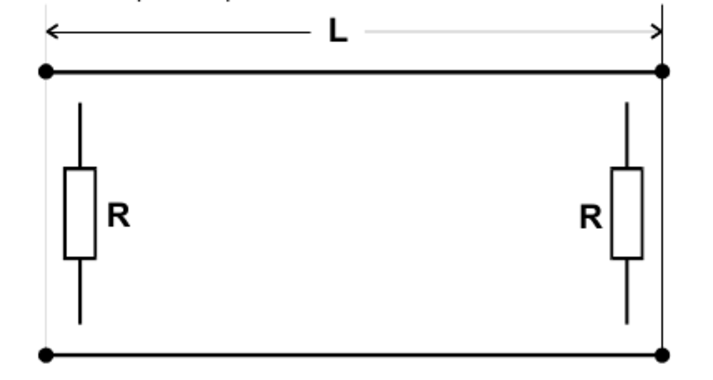
\includegraphics[width=0.8\textwidth]{figures/Doppelleitung.pdf}
  \caption{Schematisches Schaltbild einer Doppelleitung der Länge~$L$ mit zwei
  ohmschen Widerständen~\cite{V57}.}
  \label{fig:doppelleitung}
\end{figure}
%
Die Geometrie dieser Leitung legt dabei die möglichen Frequenzen der
Schwingungen fest. Somit ist auch die Anzahl~$\upD n$ der Eigenschwingungen in
einem Frequenzintervall~$\upD\nu$ festgelegt.
%
\begin{equation}
  \upD n=\frac{2L}{v_\text{Phase}}\upD\nu
\end{equation}
%
$v_\text{Phase}$ beschreibt hierbei die Phasengeschwindigkeit der Schwingung.
Der Gleichverteilungssatz der statistischen Thermodynamik ordnet nun jeder
Schwingung der Frequenz~$\nu$ eine mittlere Energie zu
%
\begin{equation}
  \upD n\bar{E}=\frac{\symup{h}\nu}{\exp{\frac{\symup{h}\nu}{\symup{k_\text{B}}T}}-1}\frac{2L}{v_\text{Phase}}\upD\nu,
\end{equation}
%
mit dem \textsc{Planck}schen Wirkungsquantum~$\symup{h}$, der
\textsc{Boltzmann}-Konstante~$\symup{k_B}$ und der Temperatur~$T$. Für die
Leistung~$P$ pro Frequenzintervall~$\upD\nu$ folgt daraus
%
\begin{equation}
  P=\frac{\symup{h}\nu}{\exp{\frac{\symup{h}\nu}{\symup{k_{\symup{B}}}T}}-1}\upD\nu.
\end{equation}
%
Wird in dem Aufbau nun berücksichtigt, dass die Widerstände Energie aus der
Schwingung absorbieren, indem sie diese in unzugängliche Wärmeenergie umwandeln,
so findet nicht mehr unbedingt eine Schwingung statt. Eine stationäre Schwingung
ist nur dann möglich, wenn die in Wärme umgewandelte Energie durch
Rauschspannungen der Widerstände ausgeglichen wird. Die maximale Leistung, die
durch das thermische Rauschen eines Widerstandes dabei zur Verfügung steht wird
durch das gemittelte Rauschstromquadrat festgelegt. Sie wird erreicht, wenn der
Wellenwiderstand~$Z$ in der Leitung dem ohmschen Widerstand~$R$ entspricht.
%
\begin{equation}
  \bar{N}_{\symup{max}}=\frac{\bar{U^2}}{4R}=P
\end{equation}
%
Das mittlere Rauschspannungsquadrat ergibt sich daraus zu
%
\begin{equation}
  \bar{U^2}(\nu)=4RP=4R\frac{\symup{h}\nu}{\exp{\frac{\symup{h}\nu}{\symup{k_{\symup{B}}}T}}-1}\upD\nu.
\end{equation}
%
Durch Näherung der Exponentialfunktion folgt schließlich die
\textsc{Nyquist}-Beziehung.
%
\begin{equation}
  \bar{U^2}=4\symup{k_{\symup{B}}}TR\upD\nu
  \label{eq:boltzmann}
\end{equation}
%
Sie beschreibt ein weißes Rauschen, also ein Rauschen, welches unabhängig von
der Breite des Frequenzbandes ist. Reale Widerstände besitzen allerdings
endliche Kapazitäten. Daraus folgt ein Einfluss auf~$Z$, sodass das
Rauschspannungsquadrat der Widerstände zusätzlich reduziert wird.

\subsection{Schrotrauschen und Schottky-Beziehung}
%
Andere Rauscheffekte treten beispielsweise bei Elektronenröhren auf. Diese
Effekte beeinflussen die Übertragung der Elektronen von der Kathode zur Anode
und lassen sich am besten im Sättigungsbetrieb\footnote{Abhängig von der
Geometrie der Röhre beschreibt der Sättigungsbetrieb den Zustand, wenn bei
ausreichender Anodenspannung alle Elektronen von der Kathode zur Anode
gelangen.} der Röhre beobachten. Hier sind nämlich folgende notwendige Annahmen
zur theoretischen Beschreibung gut erfüllt.
%
\begin{enumerate}
  \item Unabhängigkeit der Emission der einzelnen Elektronen voneinander
  \item Unabhängigkeit der Bewegung der einzelnen Elektronen voneinander
  \item Verschwindende Anfangsgeschwindigkeit der Elektronen
  \item Gleicher Weg-Zeit-Verlauf aller Elektronen (gewährleistet bei
  zylindersymmetrischer Geometrie der Röhre)
  \item Keine Sekundärelektronen an der Anode
\end{enumerate}
%
Unter diesen Annahmen lässt sich mit Hilfe des \textsc{Campbell}schen Theorems
die spektrale Verteilungsfunktion~$W_\text{Schrot}$ des Schrot-Rauschens herleiten:
%
\begin{equation}
  W_\text{Schrot}(\nu)=2e_0I_0\left\vert F(\nu)\right\vert^2.
\end{equation}
%
Dabei beschreibt~$e_0$ die Elementarladung,~$F(\nu)$ das
Frequenzspektrum des Stromimpulses und der Strom~$I_0=z\cdot e_0$
mit~$z$ als mittlere Zahl der Stromimpulse pro Zeit. Für kleine Frequenzen wird
dieser Zusammenhang unabhängig von der Frequenz und es folgt:
%
\begin{equation}
  W_\text{Schrot}=2e_0I_0.
\end{equation}
%
Das Rauschspannungsquadrat ergibt sich damit zu
%
\begin{equation}
  \bar{I^2}=2e_0I_0\upD\nu.
  \label{eq:schottky}
\end{equation}
%
Die hierfür getroffenen Annahmen 1.\,-\,5. stellen allerdings wie erwartet
Idealisierungen dar. Die Anfangsgeschwindigkeiten der Elektronen (3.) sind im
Allgemeinen nicht Null sondern folgen Verteilungen. Dies und die abschirmenden
Effekte von Sekundärelektronen in der Röhre (5.) sorgen allerdings erst bei
hohen Frequenzen für Abweichungen von der Schottky-Beziehung. Somit sind diese
Abweichungen nicht signifikant. Befindet sich die Röhre allerdings nicht im
Sättigungsbetrieb, so erzeugen entstehende Raumladungen für ein Potentialminimum
in Kathodennähe. Damit wird die Erzeugung des Rauschens durch eine so
entstehende Energieschwelle für die Elektronen unterdrückt.

\subsection{$\sfrac{1}{f}$-Rauschen: Der Funkel-Effekt}
%
Rauschprozesse, die einer Verteilung reziprok zur Frequenz der Rauschspannung
folgen und damit bei kleinen Frequenzen eine große Rolle spielen, treten in
allen elektronischen Bauteilen auf. Sie beschränken sich allerdings keineswegs
lediglich auf elektronische Prozesse. Die Gültigkeit dieser Gesetzmäßigkeit
bleibt über sehr große Frequenzbereiche bestehen und zeigt insbesondere keine
untere Grenze für kleine Frequenzen.

Ein Beispiel ist der so genannte \textbf{Funkel-Effekt}. Er tritt bei
Elektronenröhren auf, die eine Oxydkathode besitzen. Das bereits beschriebende
Schrot-Rauschen wird also von einem weiteren Rauschen überlagert. Dieses
Rauschen folgt dem Frequenzspektrum~$W_{\symup{F}}$.
%
\begin{equation}
  W_{\symup{F}}=\frac{\symup{C}}{\nu^{\alpha}}I_0^2
\end{equation}
%
Hierbei ist~$\symup{C}$ eine Konstante und~$\alpha\approx1$. Der Funkel-Effekt
stellt die Folge verschiedener phsyikalischer Prozesse dar. Hierzu gehören
atomare Diffusionsprozesse, die den Widerstand der Schicht zwischen Metallträger
und Oxydkathode lokal sprunghaft ändern. Dieser Prozess tritt besonders bei
kleinen Frequenzen auf. Die größeren Frequenzen werden durch lokale Schwankungen
der Austrittsarbeit des Oxydmaterials dominiert, die von vorübergehend an der
Oberfläche desselben absorbierten Fremdatomen herrühren.
